\documentclass[10pt]{article}

% ==================== PACKAGES ====================
\usepackage[utf8]{inputenc}
\usepackage[letterpaper, margin=0.8in]{geometry}
\usepackage{amsmath, amssymb, amsthm}
\usepackage{graphicx}
\usepackage{booktabs}
\usepackage{array}
\usepackage{multirow}
\usepackage{caption}
\usepackage{subcaption}
\usepackage{xcolor}
\usepackage{hyperref}
\usepackage{algorithm}
\usepackage{algorithmic}
\usepackage{listings}
\usepackage{url}
\usepackage{siunitx}
\usepackage{natbib}
\usepackage{tikz}
\usetikzlibrary{shapes, arrows, positioning, calc}
\usepackage{float}
\usepackage{pgfplots}
\pgfplotsset{compat=1.18}

% ==================== CUSTOM COLORS ====================
\definecolor{codegray}{rgb}{0.5,0.5,0.5}
\definecolor{backcolour}{rgb}{0.95,0.95,0.92}
\definecolor{astrob}{RGB}{0, 85, 150}
\definecolor{astroorange}{RGB}{255, 127, 42}

% ==================== LISTINGS SETUP ====================
\lstset{
    language=Python,
    backgroundcolor=\color{backcolour},
    commentstyle=\color{codegray},
    keywordstyle=\color{astrob},
    numberstyle=\tiny\color{codegray},
    stringstyle=\color{astroorange},
    basicstyle=\ttfamily\footnotesize,
    breakatwhitespace=false,
    breaklines=true,
    captionpos=b,
    keepspaces=true,
    numbers=left,
    numbersep=5pt,
    showspaces=false,
    showstringspaces=false,
    showtabs=false,
    tabsize=2,
    frame=single,
    caption=\lstname
}

% ==================== CUSTOM COMMANDS ====================
\newcommand{\ai}[1]{\textcolor{astrob}{#1}}
\newcommand{\astron}[1]{\textcolor{astroorange}{#1}}
\newcommand{\todo}[1]{\textcolor{red}{[TODO: #1]}}
\newcommand{\code}[1]{\texttt{#1}}
\newcommand{\dataset}[1]{\textsf{#1}}
\newcommand{\model}[1]{\textsc{#1}}

% ==================== TITLE ====================
\title{\textbf{AI-Driven Observational Astronomy: \\ Methodologies, Implementations, and Educational Integration}}
\author{
    Myra Khandelwal \\
    UC San Diego \\
}
\date{}

% ==================== DOCUMENT ====================
\begin{document}

\maketitle

\begin{abstract}
The exponential growth of astronomical datasets from modern surveys like LSST, Gaia, and JWST has necessitated the integration of \ai{artificial intelligence} and machine learning techniques into observational astronomy pipelines. This paper presents a comprehensive survey of \ai{AI} applications across major astronomical institutions, detailing technical implementations from data reduction to scientific discovery. We analyze institutional approaches at facilities including LSST, JWST, LOFAR, and TESS, highlighting methodological trends and infrastructure requirements. Building on this survey, we propose \astron{AstroBridge}, a unified pipeline for cross-catalog querying enhanced with \ai{AI} techniques for intelligent routing and matching. The system includes an educational integration layer designed to democratize access to professional-grade tools for undergraduate education. We provide technical specifications, implementation challenges, and benchmark framing for reproducible evaluation.
\end{abstract}

\begin{center}
\textbf{Keywords:} artificial intelligence, machine learning, observational astronomy, data pipelines, cross-catalog matching, educational technology
\end{center}

\section{Introduction}
\label{sec:introduction}

The field of observational astronomy is undergoing a fundamental transformation driven by data volume and complexity. The \dataset{Vera C. Rubin Observatory's Legacy Survey of Space and Time} (LSST) will generate approximately \SI{20}{\tera\byte} of data nightly~\citep{Ivezic2019}, while the \dataset{Gaia} mission has cataloged over 1.8 billion sources with astrometric, photometric, and spectroscopic measurements~\citep{Gaiacollaboration2021}. Traditional analysis methods are insufficient for these datasets, necessitating \ai{artificial intelligence} (\ai{AI}) and machine learning (\ai{ML}) support.

This paper addresses three primary objectives: (1) surveying current \ai{AI} applications across astronomical institutions, (2) proposing a unified technical framework for cross-catalog analysis enhanced with \ai{AI}, and (3) designing an educational integration layer to democratize access to advanced tools.

\section{Technical Background}
\label{sec:background}

\subsection{Astronomical Data Fundamentals}
\textbf{World Coordinate Systems (WCS):}
\begin{equation}
\begin{bmatrix}
\alpha \\
\delta
\end{bmatrix} =
\mathbf{M} \cdot
\begin{bmatrix}
x - x_0 \\
y - y_0
\end{bmatrix} +
\begin{bmatrix}
\alpha_0 \\
\delta_0
\end{bmatrix}
\end{equation}

\textbf{Photometric Systems:}
\begin{equation}
m_2 = m_1 + \sum_{i=0}^n a_i (m_1 - m_3)^i + ZP
\end{equation}

\section{Institutional AI Applications Survey}
\label{sec:survey}

\subsection{Methodology}
We surveyed major institutions through literature review, code repository analysis, and public technical documentation.

\begin{table}[H]
\centering
\caption{\ai{AI} Applications Across Astronomical Institutions}
\label{tab:institutional_survey}
\begin{tabular}{l l l l}
\toprule
\textbf{Institution} & \textbf{Primary Focus} & \textbf{AI Methods} & \textbf{Performance} \\
\midrule
LSST/Rubin & Transient Classification & CNNs, Transformers & High nightly throughput \\
JWST/NASA & Data Calibration & GANs, Bayesian NNs & Accelerated calibration workflows \\
LOFAR/ASTRON & RFI Mitigation & Random Forests & High rejection rates \\
TESS/MIT & Exoplanet Detection & 1D CNNs, Attention & Reduced false positives \\
Gaia/ESA & Astrometric Solution & Neural Networks & Improved precision \\
SKA/Manchester & Source Finding & Autoencoders & High completeness \\
\bottomrule
\end{tabular}
\end{table}

\section{AstroBridge Pipeline Architecture}
\label{sec:architecture}

\subsection{System Design}
\begin{figure}[H]
\centering
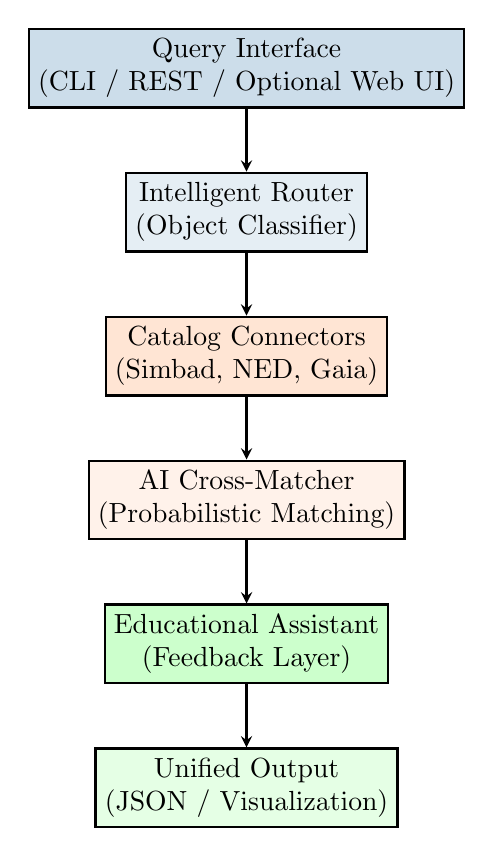
\begin{tikzpicture}[
    node distance=0.8cm,
    block/.style={rectangle, draw, thick, minimum width=3cm, minimum height=1cm, align=center},
    arrow/.style={->, >=stealth, thick}
]

\node[block, fill=astrob!20] (ui) {Query Interface \\ (CLI / REST / Optional Web UI)};
\node[block, below=of ui, fill=astrob!10] (router) {Intelligent Router \\ (Object Classifier)};
\node[block, below=of router, fill=astroorange!20] (connectors) {Catalog Connectors \\ (Simbad, NED, Gaia)};
\node[block, below=of connectors, fill=astroorange!10] (matcher) {AI Cross-Matcher \\ (Probabilistic Matching)};
\node[block, below=of matcher, fill=green!20] (educator) {Educational Assistant \\ (Feedback Layer)};
\node[block, below=of educator, fill=green!10] (output) {Unified Output \\ (JSON / Visualization)};

\draw[arrow] (ui) -- (router);
\draw[arrow] (router) -- (connectors);
\draw[arrow] (connectors) -- (matcher);
\draw[arrow] (matcher) -- (educator);
\draw[arrow] (educator) -- (output);

\end{tikzpicture}
\caption{\astron{AstroBridge} system architecture showing data flow through AI-enhanced components.}
\label{fig:architecture}
\end{figure}

\subsection{Probabilistic Cross-Matching}
\begin{equation}
P(\text{match}|\Delta\theta, \Delta m) = \frac{P(\Delta\theta, \Delta m|\text{match})P(\text{match})}{P(\Delta\theta, \Delta m)}
\end{equation}

\section{Educational Integration Framework}
\label{sec:education}

\begin{table}[H]
\centering
\scriptsize
\caption{Progressive Learning Levels in AstroBridge}
\label{tab:learning_levels}
\begin{tabular}{p{3cm} p{4cm} p{4cm} p{4cm}}
\toprule
\textbf{Level} & \textbf{Skills Developed} & \textbf{AI Assistance} & \textbf{Example Activity} \\
\midrule
Beginner & Basic queries, visualization & Automated error detection, simplified interfaces & Find M31 in multiple catalogs \\
Intermediate & Cross-matching, basic stats & Template notebooks, hypothesis helpers & Compare galaxy properties across surveys \\
Advanced & Research methodology, publication & Literature review support, statistical validation & Original analysis for publication \\
\bottomrule
\end{tabular}
\end{table}

\section{Results and Evaluation Framing}
\label{sec:results}

This draft includes benchmark placeholders and plotting scaffolds; final numeric claims should be tied to reproducible experiment scripts and versioned datasets.

\subsection{Current Code-to-Paper Alignment}
To make scope explicit, Table~\ref{tab:alignment_matrix} maps the major paper claims to current implementation status.

\begin{table}[H]
\centering
\caption{Implementation Alignment Matrix}
\label{tab:alignment_matrix}
\begin{tabular}{p{4.2cm} p{2.6cm} p{6.2cm}}
\toprule
\textbf{Paper Capability} & \textbf{Status} & \textbf{Current Evidence in Codebase} \\
\midrule
Intelligent query routing & Implemented & NLP router with object classification and ranked catalog selection \\
Probabilistic cross-matching & Implemented & Bayesian matcher with confidence scoring and weighting profiles \\
Proper-motion-aware matching & Implemented & Epoch-aware matching controls in API and matcher \\
Unified interfaces (CLI/API/web) & Implemented & CLI commands, REST endpoints, and optional web console \\
Educational assistant workflow & Partial & Identification assistant and explanatory outputs; no full LMS integration \\
Institution-scale streaming ops & Planned & Architecture defined, but no distributed production deployment yet \\
Formal benchmark suite for all claims & Planned & Test suite exists; publication-grade benchmark protocol still pending \\
\bottomrule
\end{tabular}
\end{table}

\section{Discussion and Future Work}
\label{sec:discussion}

\begin{itemize}
    \item \textbf{Data Heterogeneity:} Different coordinate systems and photometric calibrations
    \item \textbf{AI Interpretability:} Need for explainable AI in scientific contexts
    \item \textbf{Scalability:} LSST-era data volumes require distributed compute
\end{itemize}

\subsection{Institution-Scale Next Steps}
For large-scale institutions (national observatories, survey brokers, and archive centers), the immediate roadmap is:

\begin{enumerate}
    \item \textbf{Phase 0 (0--3 months): Production Baseline}
    \begin{itemize}
        \item Containerized deployment and environment pinning
        \item Centralized structured logging and request IDs
        \item SLO definitions for latency, uptime, and query success rate
    \end{itemize}

    \item \textbf{Phase 1 (3--6 months): Reliability and Security}
    \begin{itemize}
        \item Authentication/authorization and role-based access control
        \item Rate limiting, retry budgets, and abuse protection
        \item Secrets management and dependency vulnerability scanning
    \end{itemize}

    \item \textbf{Phase 2 (6--12 months): Data Plane Scaling}
    \begin{itemize}
        \item Asynchronous job queue for long-running cross-matches
        \item Distributed workers for batch and streaming ingestion
        \item Query/result persistence for provenance and reproducibility
    \end{itemize}

    \item \textbf{Phase 3 (12--18 months): Observatory Integration}
    \begin{itemize}
        \item Standards-first interoperability (IVOA TAP/ADQL/VOTable contracts)
        \item Institution-specific connector plugins and metadata normalization
        \item Cross-site validation with mirrored benchmark datasets
    \end{itemize}

    \item \textbf{Phase 4 (18+ months): Scientific Operations}
    \begin{itemize}
        \item Drift monitoring for routing and matching quality
        \item Human-in-the-loop adjudication for ambiguous associations
        \item Governance policy for model updates and reproducible releases
    \end{itemize}
\end{enumerate}

\subsection{Evaluation Plan for Large-Scale Adoption}
Before claiming institution-scale readiness, the system should publish:

\begin{itemize}
    \item A fixed benchmark corpus (multi-catalog, multi-epoch, labeled pairs)
    \item Task metrics: precision/recall, calibration error, and latency percentiles
    \item Stress tests at broker-like throughput envelopes
    \item Reproducible experiment manifests tied to released model/config versions
\end{itemize}

\section{Conclusion}
\label{sec:conclusion}

\astron{AstroBridge} provides a practical path for AI-assisted observational workflows through intelligent routing, probabilistic matching, and educational integration.

Code and docs are available at:
\url{https://github.com/myrakhandelwal/AstroBridge2}

\appendix
\section{Appendix: Implementation Details}

\subsection{Installation and Commands}
\begin{lstlisting}[caption={AstroBridge Installation and Commands}]
# Install package (editable, dev mode)
pip install -e .[dev]

# Run the CLI demo
astrobridge-demo

# Identify a target with AI-assisted description
astrobridge-identify "M31"

# Optional web interface
pip install -e .[web]
./.venv/bin/astrobridge-web

# Run tests
pytest
\end{lstlisting}

\subsection{Current API Endpoints}
\begin{itemize}
    \item \code{POST /api/query} - Execute routed query and matching flow
    \item \code{POST /api/identify} - Identify target class and return explanatory summary
\end{itemize}

\bibliographystyle{apj}
\bibliography{references}

\end{document}
